\section{Architectural Diagram}

\subsection{Main Design}

The system will be designed with three separate major isolated systems, running in different locations/with differing levels of access from company mining sites. The vehicle API will be on board the vehicle ECUs and interfaces with the existing ECU firmware to extract sensor data from the ECU and ``push'' it to the gateway. Before sending the vehicle data to the gateway, some pre-processing and conversion occur on-board the vehicle ECU API and then the message is sent via a push architecture to the gateway. This was chosen so that when a vehicle is flashed with its firmware, the messages it reports will be of a standard form and recognizable units of that of other vehicles (also flashed with appropriate VAPI firmware). Subsequent changes to firmware (that could affect sensor messages) are easily accounted for and changes to the VAPI can be made, tracked, and version controlled in the same repository. Finally, a push architecture is used to simplify the protocol between the gateway and the vehicle.

The vehicle gateway is the second device, serving as the primary system for which vehicles can communicate their onboard diagnostic data with the other company services. This gateway is designed to simply forward and publish messages as appropriate when messages are received from vehicles and requires little to no computation power, and simply an up-link to perform its main task. The simplicity of the gateway is such as it is a single point of failure between the vehicles and the health reporting backend of the system, thus it must be simple and easy to replace or add redundancy to if needed.\newpage

Finally, the third system is hosted on the cloud. While it is possible to have it on-premise on server racks, this architecture allocates off-premise infrastructure for metric collection, monitoring, and web-view hosting. This was to make the system easily accessible from a variety of locations and remove complexity involved with installing this on local, on-site hardware.

\subsubsection{Context Diagram}

\begin{figure}[H]
\centering
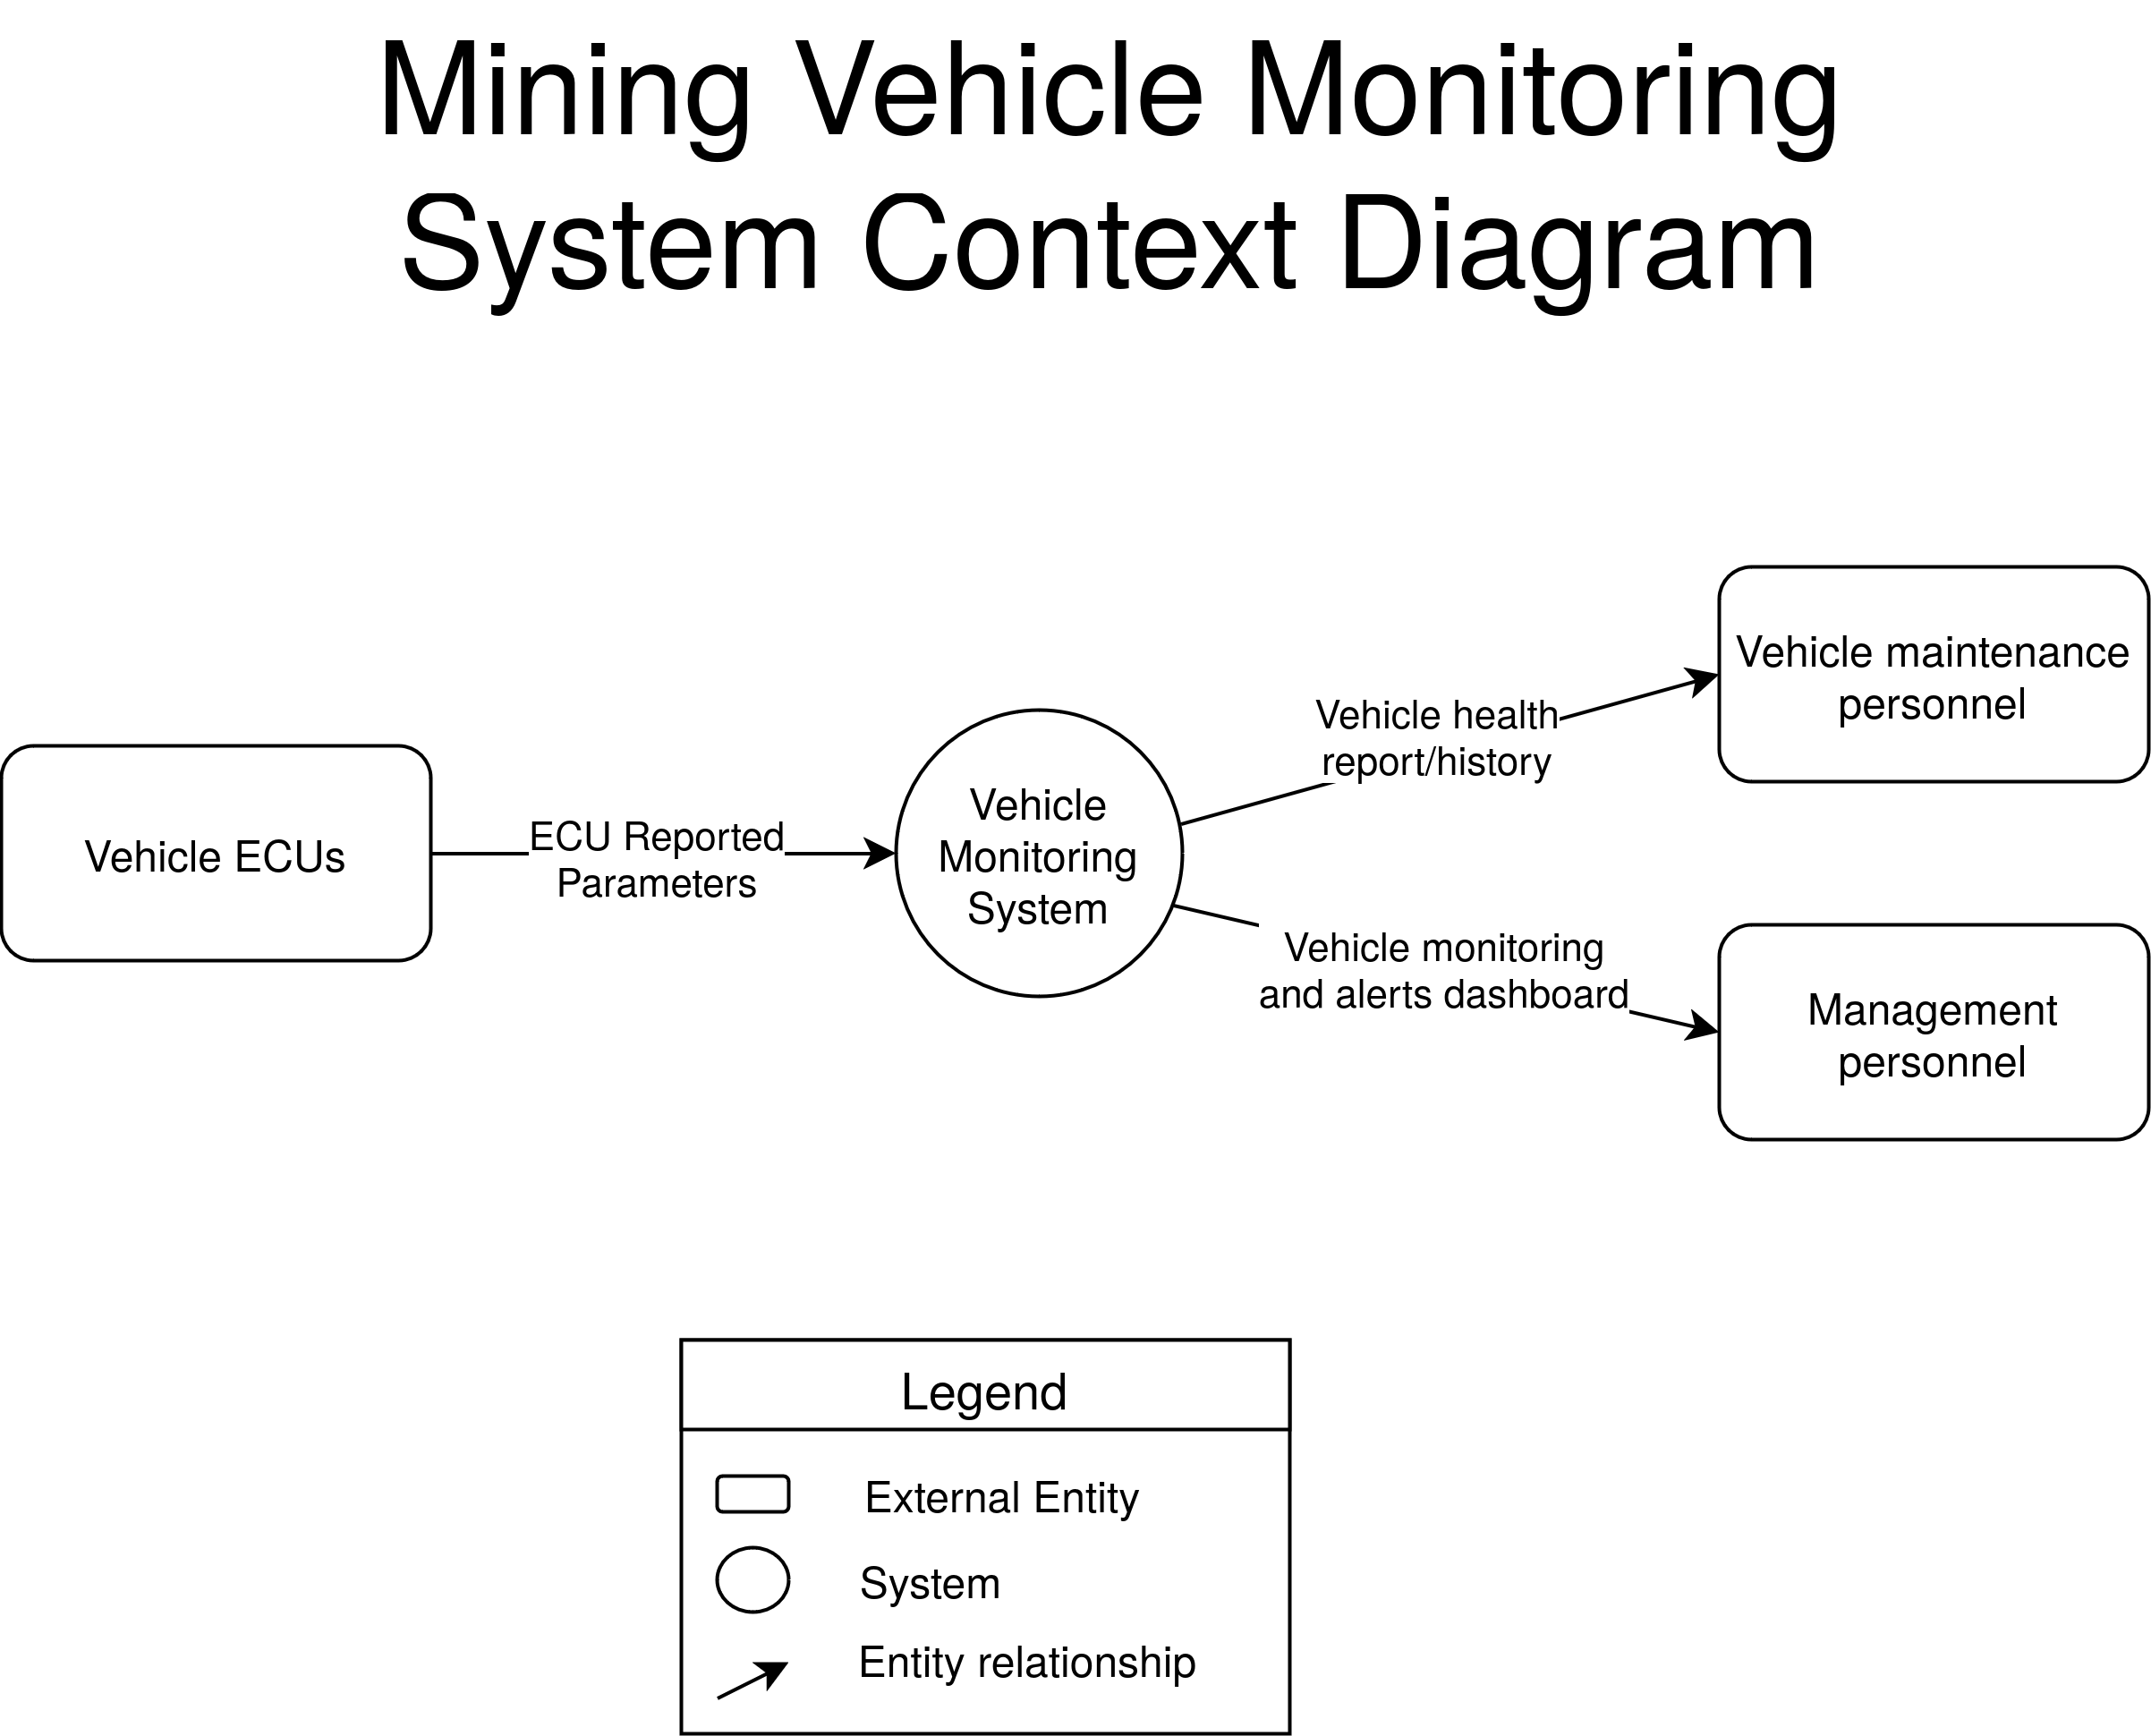
\includegraphics[width=0.8\textwidth]{Images/project-context-diagram.png}
\caption{Context Diagram of system}
\label{fig:system_context_diagram}
\end{figure}

\subsubsection{Dynamic View - Allocation}

\begin{figure}[H]
\centering
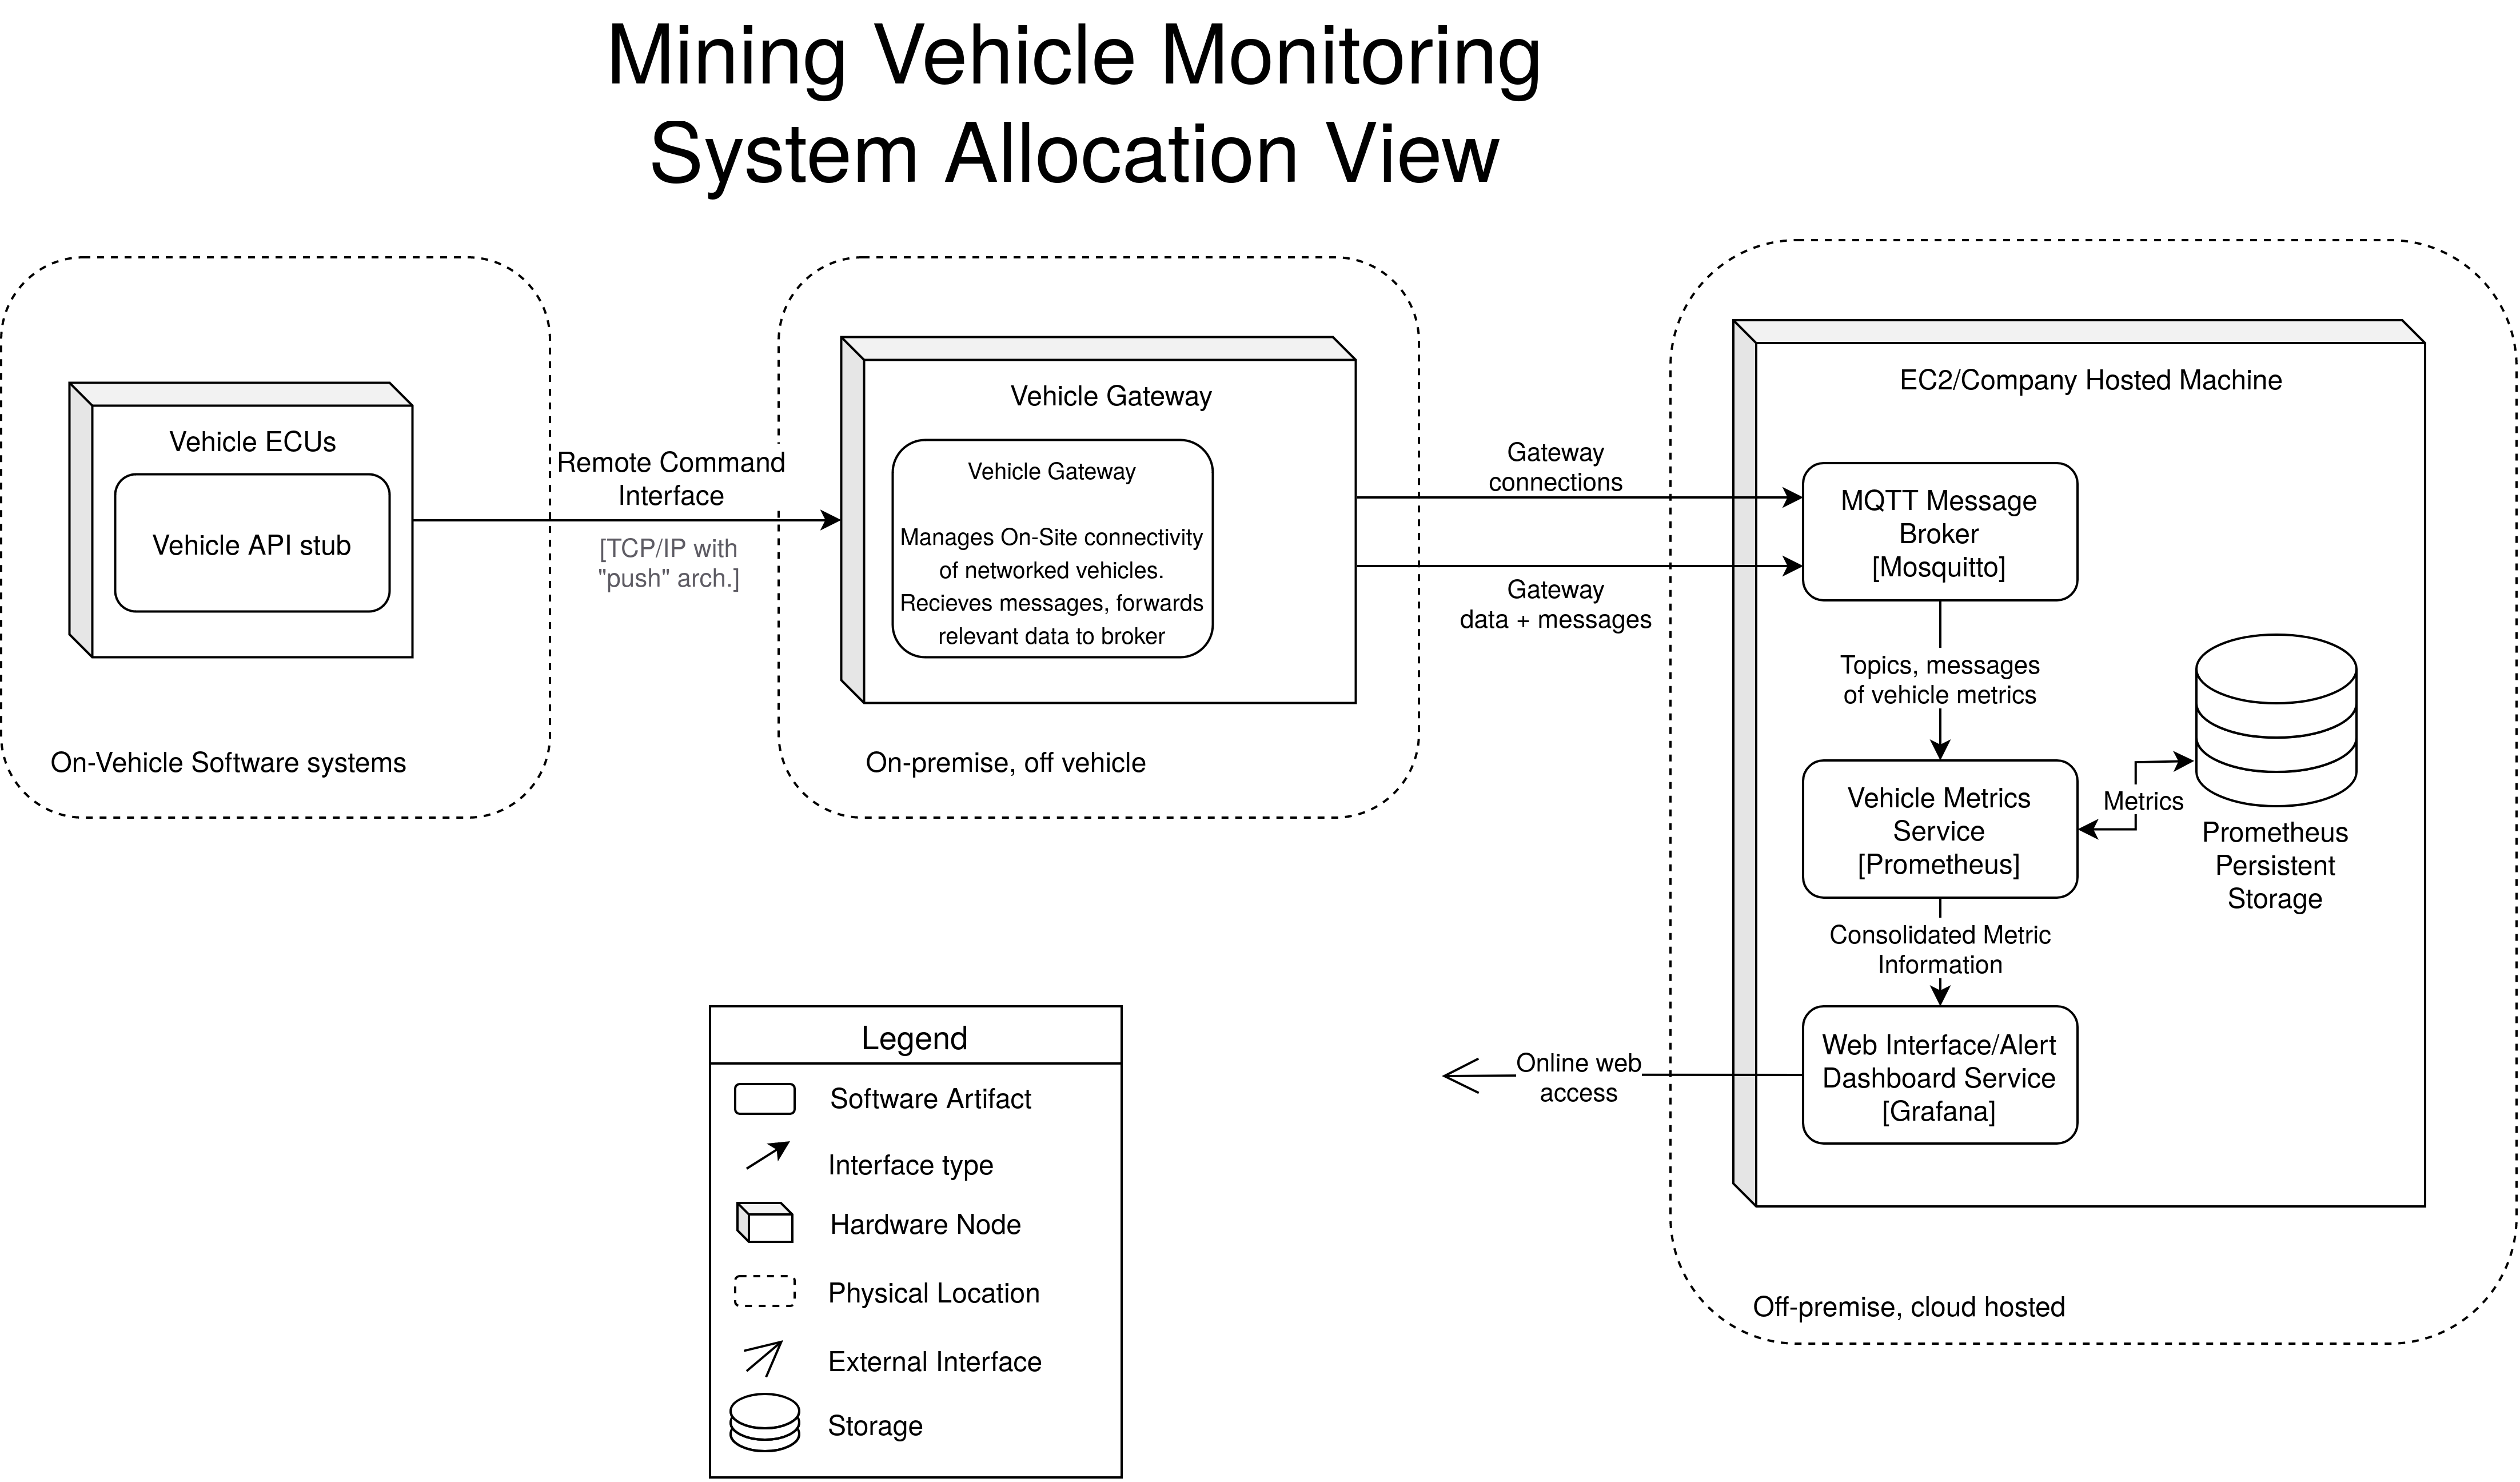
\includegraphics[width=0.8\textwidth]{Images/project-allocation-view.png}
\caption{Allocation view of system}
\label{fig:allocation_view}
\end{figure}

\begin{figure}[H]
\centering
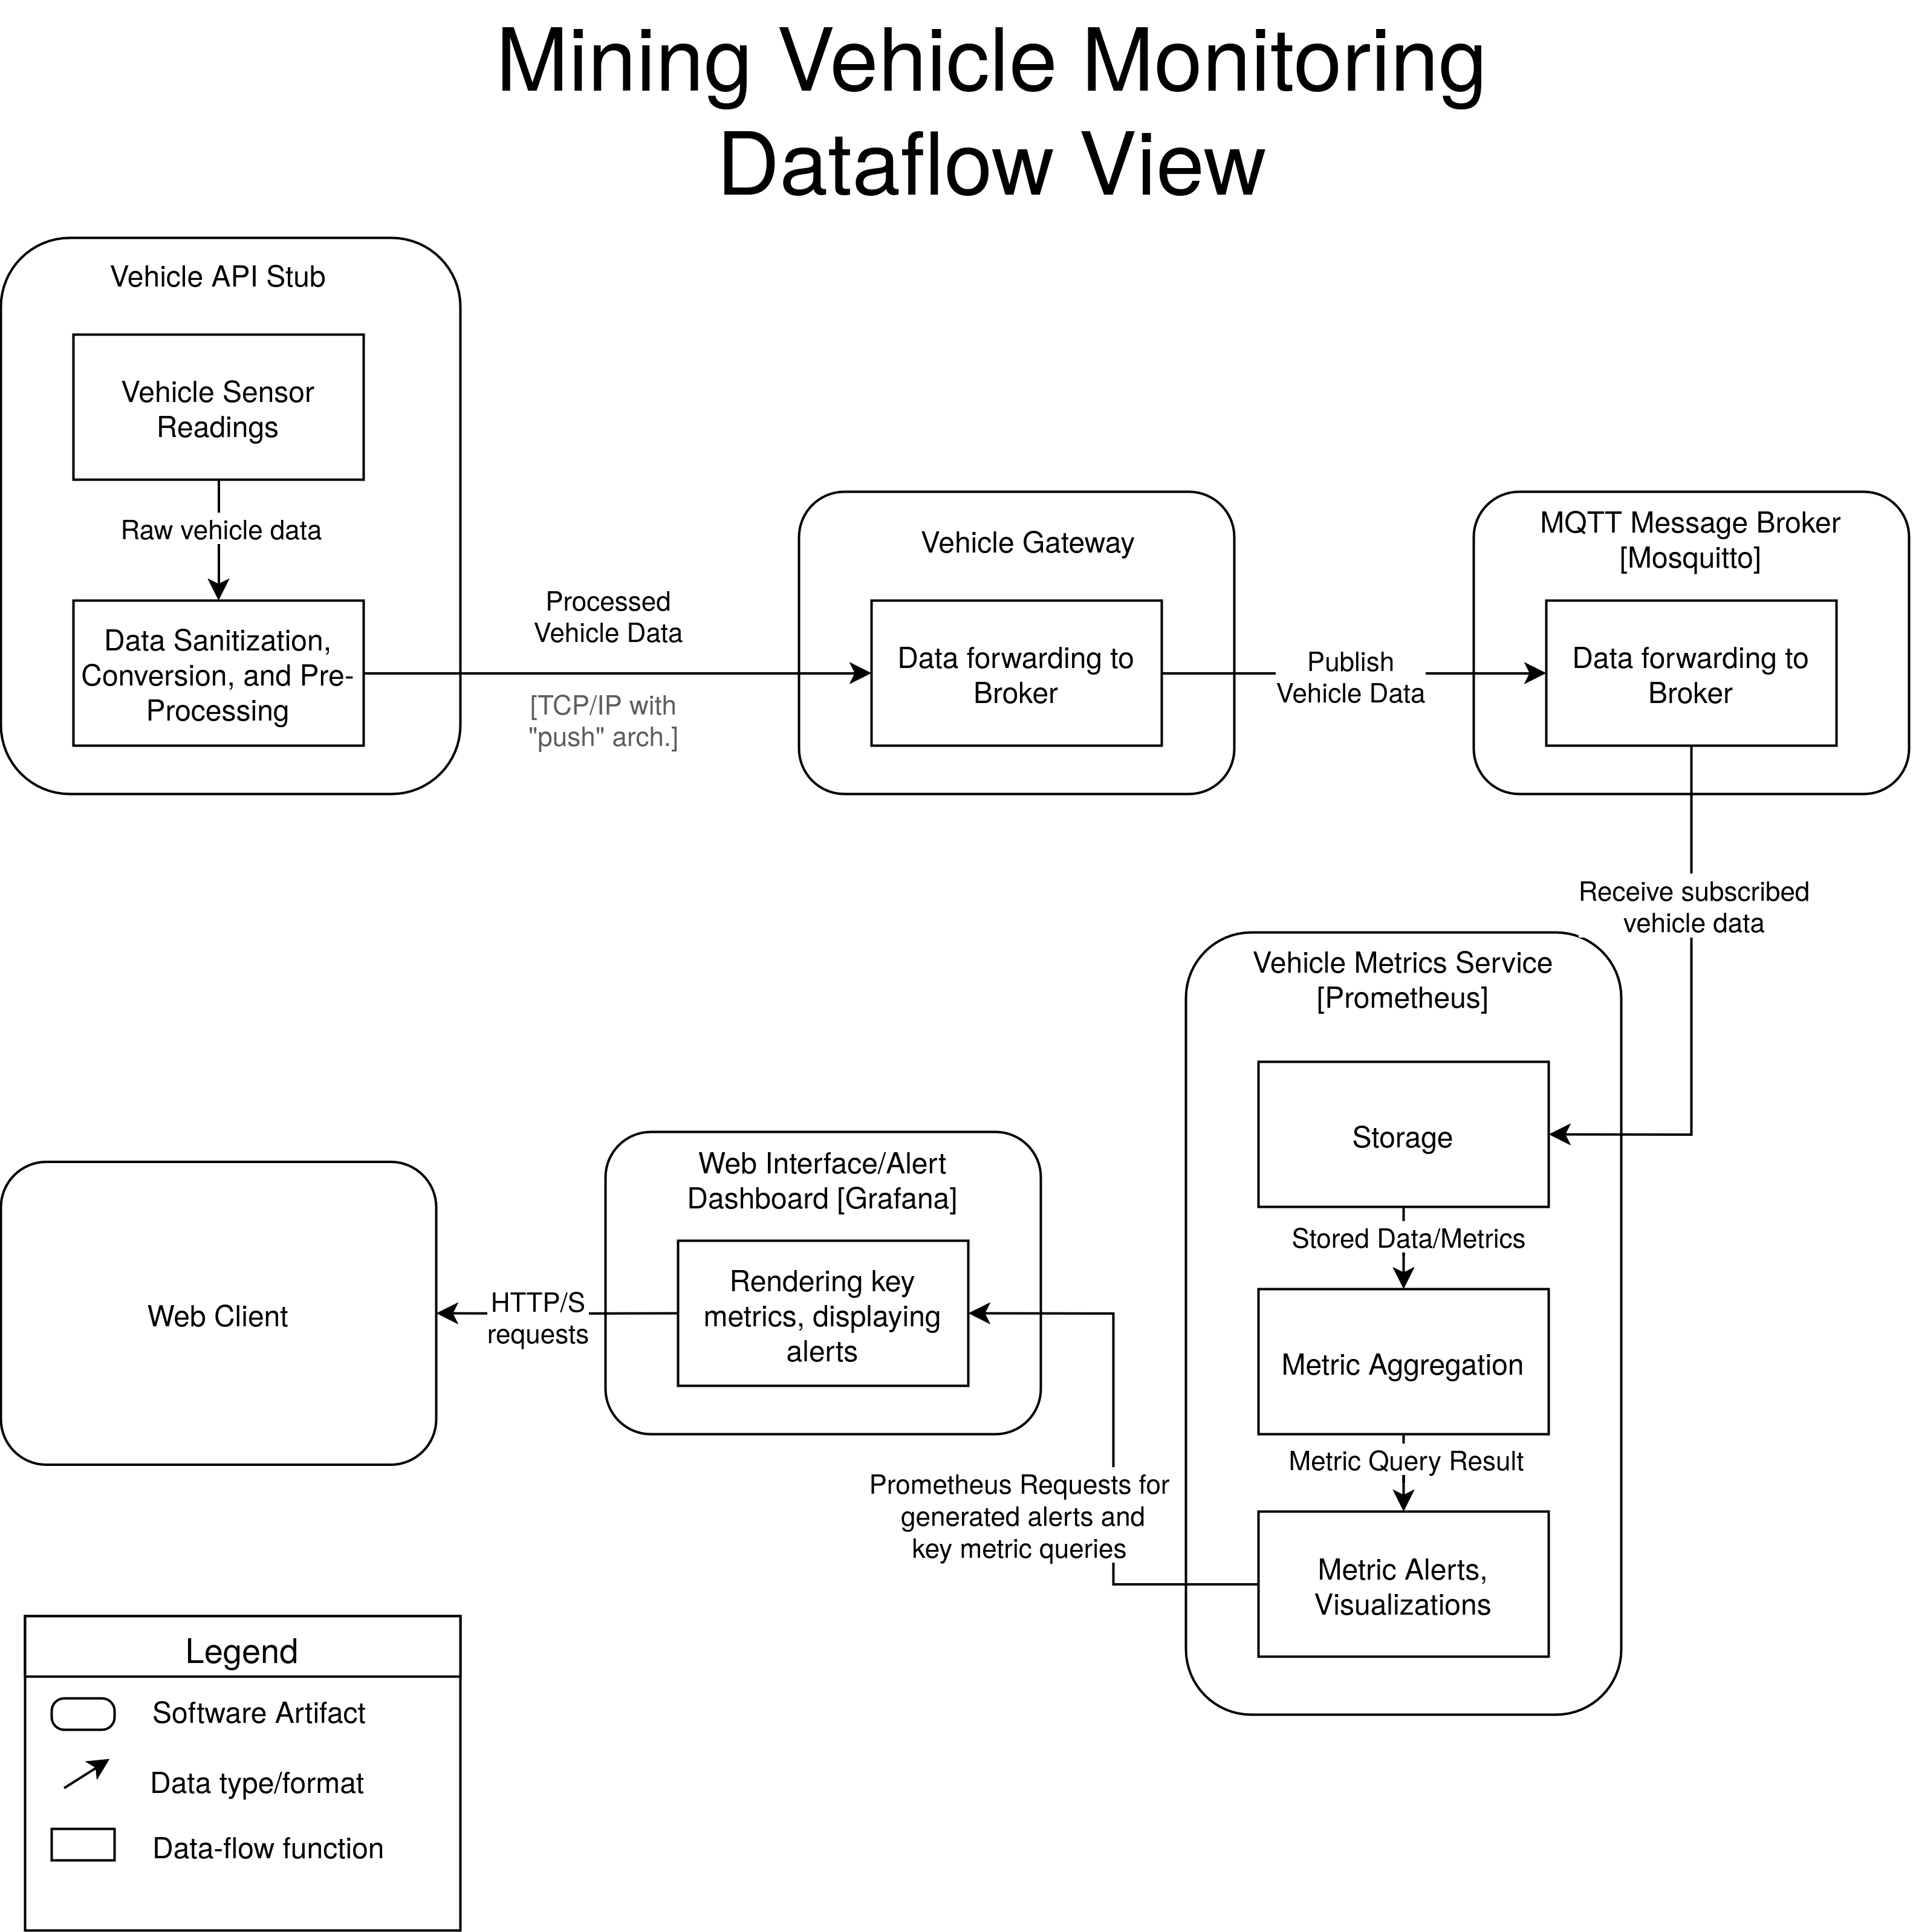
\includegraphics[width=0.8\textwidth]{Images/project-dataflow-view.png}
\caption{Dataflow view of system}
\label{fig:dataflow_view}
\end{figure}

\pagebreak
\subsection{Component Catalog}
\begin{table}[H]
\begin{tabular}{|l|p{0.65\textwidth}|}
\hline
Component Name                & Description \\ \hline \hline
Vehicle API Stub              & Small bit of onboard code that interfaces with rest of vehicle ECU. Obtains relevant sensor data from the vehicle, perform pre-processing steps, and the sends data to gateway in a ``push'' style architecture. \\ \hline
Vehicle Gateway               & Simple gateway acting as barrier and coordinator between vehicles and external services. Forwards messages sent from vehicles to MQTT broker. \\ \hline
MQTT Message Broker           & Receives vehicle messages published and notifies MQTT subscribers of new vehicle metrics - generally the main subscriber will be the Metrics service. Built using Mosquitto. \\ \hline
Vehicle Metrics Service       & Collects, stores, aggregrates published metrics from MQTT channel into backend database for further processing, searching, and extraction of alerts. Built using Prometheus. \\ \hline
Web Interface/Alert Dashboard & Queries metrics service for relevant alerts, key metrics and data, and time series information about the health of the machines. Built using Grafana.\\ \hline
Cloud-Hosted Machine          & An off-premise machine accessible via its Grafana web interface for end users or can be serviced remotely via ssh, or an equivalent. Likely runs the 3 prior services in containers or VMs on instance. \\ \hline   
\end{tabular}
\end{table}


% Figure \ref{fig:overengineered_paperclip} shows a schematic diagram of an over engineered paperclip which serves as an example to the time-honored engineering tradition of fixing what isn't broken.

% This is a great place to throw a random citation \cite{author2020} to make it look like I've read the literature.